\documentclass{article}

\usepackage{amsmath}
\usepackage{amssymb}
\usepackage{algorithm}
\usepackage[noend]{algpseudocode}		% for algorithms in pseudo code. Usage: \begin{algorithmic}
\MakeRobust{\Call}
\usepackage{tikz}	% for diagrams
\usetikzlibrary{positioning}
\usetikzlibrary{quotes}

\setlength{\parskip}{\smallskipamount}

\title{Analysis of Algorithms \\
\medskip
\large Homework 3}
\author{Abraham Murciano}

\begin{document}

\maketitle

\section{The Kruskal and Prim Algorithms}

We are given the following weighted, undirected graph \(G = (V, E)\) where \(V\) is the set of vertices, \(E\) is a set of edges, and \(w_{u,v}\) is the weight from vertices \(u\) to \(v\).
\begin{gather*}
	V = \{a, b, c, d, e, f, g, h, i\} \\
	E = \{\{a, b\}, \{a, h\}, \{a, i\}, \{b, c\}, \{b, f\}, \{c, d\}, \{d, e\},\\ \{d, g\}, \{d, h\}, \{e, f\}, \{f, g\}, \{h, i\}\} \\
	w_{a, b} = 4, w_{a, h} = 10, w_{a, i} = 6, w_{b, c} = 7, w_{b, f} = 12, w_{c, d} = 8, w_{d, e} = 3, \\ w_{d, g} = 5, w_{d, h} = 2, w_{e, f} = 11, w_{f, g} = 1, w_{h, i} = 9)
\end{gather*}

\subsection{Kruskal}

We are to run the Kruskal algorithm on this graph, showing intermediate stages. We begin with the set of edges to return \(F\), initialised to \(\phi\). We also begin with a disjoint set \(D\), starting with each vertex in its own set; i.e \(D = \{\{v\} : v \in V\}\).

The set the algorithm returns as a minimum spanning forrest is
\begin{equation*}
	F = \{\{a, b\}, \{a, i\}, \{b, c\}, \{c, d\}, \{d, e\}, \{d, g\}, \{d, h\}, \{f, g\}\}
\end{equation*}
as shown by the intermediate steps in table \ref{q1a-steps}.

\begin{table}[htbp]
	\centering
	\begin{tabular}{|c|c|c|}
		\hline
		Step & Variable & Value \\
		\hline
		1    & \(F\)    & \(\{\{f, g\}\}\) \\
		     & \(D\)    & \(\{\{a\}, \{b\}, \{c\}, \{d\}, \{e\}, \{f, g\}, \{h\}, \{i\}\}\) \\
		\hline
		2    & \(F\)    & \(\{\{d, h\}, \{f, g\}\}\) \\
		     & \(D\)    & \(\{\{a\}, \{b\}, \{c\}, \{d, h\}, \{e\}, \{f, g\}, \{i\}\}\) \\
		\hline
		3    & \(F\)    & \(\{\{d, e\}, \{d, h\}, \{f, g\}\}\) \\
		     & \(D\)    & \(\{\{a\}, \{b\}, \{c\}, \{d, e, h\}, \{f, g\}, \{i\}\}\) \\
		\hline
		4    & \(F\)    & \(\{\{a, b\}, \{d, e\}, \{d, h\}, \{f, g\}\}\) \\
		     & \(D\)    & \(\{\{a, b\}, \{c\}, \{d, e, h\}, \{f, g\}, \{i\}\}\) \\
		\hline
		5    & \(F\)    & \(\{\{a, b\}, \{d, e\}, \{d, g\}, \{d, h\}, \{f, g\}\}\) \\
		     & \(D\)    & \(\{\{a, b\}, \{c\}, \{d, e, f, g, h\}, \{i\}\}\) \\
		\hline
		6    & \(F\)    & \(\{\{a, b\}, \{a, i\}, \{d, e\}, \{d, g\}, \{d, h\}, \{f, g\}\}\) \\
		     & \(D\)    & \(\{\{a, b, i\}, \{c\}, \{d, e, f, g, h\}\}\) \\
		\hline
		7    & \(F\)    & \(\{\{a, b\}, \{a, i\}, \{b, c\}, \{d, e\}, \{d, g\}, \{d, h\}, \{f, g\}\}\) \\
		     & \(D\)    & \(\{\{a, b, c, i\}, \{d, e, f, g, h\}\}\) \\
		\hline
		8    & \(F\)    & \(\{\{a, b\}, \{a, i\}, \{b, c\}, \{c, d\}, \{d, e\}, \{d, g\}, \{d, h\}, \{f, g\}\}\) \\
		     & \(D\)    & \(\{\{a, b, c, d, e, f, g, h, i\}\}\) \\
		\hline
	\end{tabular}
	\caption{The steps taken during the execution of the Kruskal algorithm}
	\label{q1a-steps}
\end{table}

\subsection*{Prim}

Using the same example we are to run Prim's algorithm which returns the same thing. We start with an set of vertices \(V_0\) initialised to an arbitrary vertex (here we choose \(a\)), which we insert vertices into one at a time. We also use a set \(E_0\) which is the subset of edges to return, initialised to \(\phi\). By the end,
\begin{equation*}
	E_0 = \{\{a, b\}, \{a, i\}, \{b, c\}, \{c, d\}, \{d, e\}, \{d, g\}, \{d, h\}, \{f, g\}\}
\end{equation*}


\begin{table}[htbp]
	\centering
	\begin{tabular}{|c|c|c|}
		\hline
		Step & Variable & Value \\
		\hline
		1    & \(V_0\)  & \(\{a\}\) \\
		     & \(E_0\)  & \(\phi\) \\
		\hline
		2    & \(V_0\)  & \(\{a, b\}\) \\
		     & \(E_0\)  & \(\{\{a, b\}\}\) \\
		\hline
		3    & \(V_0\)  & \(\{a, b, i\}\) \\
		     & \(E_0\)  & \(\{\{a, b\}, \{a, i\}\}\) \\
		\hline
		4    & \(V_0\)  & \(\{a, b, c, i\}\) \\
		     & \(E_0\)  & \(\{\{a, b\}, \{a, i\}\}, \{b, c\}\) \\
		\hline
		5    & \(V_0\)  & \(\{a, b, c, d, i\}\) \\
		     & \(E_0\)  & \(\{\{a, b\}, \{a, i\}\}, \{b, c\}, \{c, d\}\) \\
		\hline
		6    & \(V_0\)  & \(\{a, b, c, d, h, i\}\) \\
		     & \(E_0\)  & \(\{\{a, b\}, \{a, i\}\}, \{b, c\}, \{c, d\}, \{d, h\}\) \\
		\hline
		7    & \(V_0\)  & \(\{a, b, c, d, e, h, i\}\) \\
		     & \(E_0\)  & \(\{\{a, b\}, \{a, i\}\}, \{b, c\}, \{c, d\}, \{d, e\}, \{d, h\}\) \\
		\hline
		8    & \(V_0\)  & \(\{a, b, c, d, e, g, h, i\}\) \\
		     & \(E_0\)  & \(\{\{a, b\}, \{a, i\}\}, \{b, c\}, \{c, d\}, \{d, e\}, \{d, g\}, \{d, h\}\) \\
		\hline
		9    & \(V_0\)  & \(\{a, b, c, d, e, f, g, h, i\}\) \\
		     & \(E_0\)  & \(\{\{a, b\}, \{a, i\}, \{b, c\}, \{c, d\}, \{d, e\}, \{d, g\}, \{d, h\}, \{f, g\}\}\) \\
		\hline
	\end{tabular}
	\caption{The steps taken during the execution of the Prim algorithm}
	\label{q1b-steps}
\end{table}

\section{Minimal Spanning Trees and Shortest Paths}

It is not necessarily true that the path between any two vertices on a minimal spanning tree of a graph is also a shortest path between these two vertices on this graph. As a counter-example, suppose we have the following graph.
\begin{gather*}
	V = \{a, b, c\} \\
	E = \{\{a, b\}, \{b, c\}, \{a, c\}\} \\
	w_{a,b} = 2, w_{b, c} = 2, w_{a,c} = 3
\end{gather*}

Here, the shorted path between \(a\) and \(c\) is the single edge \(\{a, c\}\) of weight 3, however the path between them in the minimal spanning tree is of weight 4.

\section{Finding the Maximal Spanning Tree}

We are to write an algorithm to find the maximal spanning tree of a graph. The algorithm presented below is a slight modification of Kruskal's algorithm, where instead of sorting the edges by increasing weight, we sort them by decreasing weight.

\begin{algorithm}
	\begin{algorithmic}
		\Function{MaximalSpanningTree}{$V, E$}
		\State \(F := \phi\)
		\State \(D := \Call{DisjointSet}{V}\)
		\State Sort \(E\) by decreasing weight
		\For{\((u, v) \in E\)}
		\If{\(D.\Call{FindSet}{u} \neq D.\Call{FindSet}{v}\)}
		\State \(F := F \cup \{(u, v)\}\)
		\State \(D.\Call{Union}{D.\Call{FindSet}{u}, D.\Call{FindSet}{v}}\)
		\EndIf
		\EndFor
		\State \Return \(F\)
		\EndFunction
	\end{algorithmic}
\end{algorithm}

The proof of its correctness is the same logic as that for Kruskal's algorithm, and its complexity is identical, namely \(O(E\alpha(V))\), where \(\alpha\) is the inverse Ackermann function. It uses \(O(V)\) extra space because \(D\) uses \(O(V)\) space, and the maximal spanning tree contains \(|V| - 1\) edges.

\section{Propositions on Minimal Spanning Trees}

For each of the following propositions we are to prove or disprove them. Let \(G = (V, E)\) be a connected undirected weighted graph.

\begin{enumerate}
	\item
		\(G\) has only one minimal spanning tree.

		\paragraph{Disproof.} This statement is false, as shown in the counter-example in figure \ref{q4a-counter}. Since all three edges are the same weight, and any two of them form a spanning tree, there are three distinct spanning trees, which are all minimal.
		\begin{figure}[htbp]
			\centering
			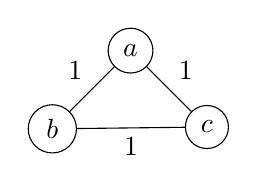
\begin{tikzpicture}
				[vertex/.style={circle, draw=black, node distance=0.8cm}]
				\node[vertex] (a) {\(a\)};
				\node[vertex, below left=of a] (b)  {\(b\)};
				\node[vertex, below right=of a] (c) {\(c\)};
				\draw (a) to["{1}" above left] (b);
				\draw (a) to["{1}" above right] (c);
				\draw (b) to["{1}" below] (c);
			\end{tikzpicture}
			\caption{A graph with three different minimal spanning trees}
			\label{q4a-counter}
		\end{figure}

	\item
		If all the weights in \(G\) are different, then there exists only one minimal spanning tree.

		\paragraph{Proof.} This proposition is true. We shall prove it by contradiction. Suppose the contrary; i.e. there exist two minimal spanning trees \(S\) and \(T\) such that \(S \neq T\). Let \(e\) be the edge with the smallest weight in \(S\) which is not in \(T\), or vice versa. (Without loss of generality, suppose \(e \in S\).)

		If we add \(e\) to \(T\), we obtain a graph \(T_1\) with a cycle. This cycle must contain some other edge \(f\) which is not in \(S\), and we know that \(w_e < w_f\), since we chose \(e\) to be the smallest edge which was not common to \(S\) and \(T\), and all the edges are of different sizes.

		Therefore we can define \(T_2\) as the graph obtained if we remove \(f\) from \(T_1\). This breaks the only cycle in \(T_1\), meaning \(T_2\) is a tree. It spans the same vertices that \(T_1\) spans, which are the same vertices that \(T\) spans, so since \(T\) spans the entire graph, so does \(T_2\). Finally, the total weight of the edges in \(T_2\) is smaller than that of \(T\), since \(T_2\) only differs by having \(e\) instead of \(f\), which has a smaller weight.

		Thus we have shown that there exists a smaller spanning tree than \(T\), which contradicts \(T\)'s minimality. Therefore we can conclude that there cannot be two minimal spanning trees if the weights are all different.

	\item
		If \(G\) has two edges of the same weight, then there must be at least two minimal spanning trees.

		\paragraph{Disproof.} This can be disproven with a counter-example as shown in figure \ref{q4c-counter}.

		\begin{figure}[htbp]
			\centering
			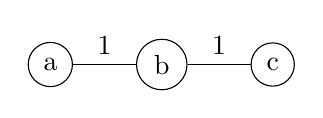
\begin{tikzpicture}
				[vertex/.style={circle, draw=black, node distance=0.8cm}]
				\node[vertex] (a) {a};
				\node[vertex, right=of a] (b) {b};
				\node[vertex, right=of b] (c) {c};
				\draw (a) to["{1}" above] (b);
				\draw (b) to["{1}" above] (c);
			\end{tikzpicture}
			\caption{A graph with two edges of the same weight and only one minimal spanning tree}
			\label{q4c-counter}
		\end{figure}
\end{enumerate}

\section{More Proofs on Spanning Trees}

\begin{enumerate}
	\item
		Each connected undirected graph \(G=(V,E)\) has a spanning tree.

		\paragraph{Proof.} A spanning tree is a connected subgraph which contains every vertex but no cycles. \(G\) itself is connected (thus spans all the vertices), but may contain cycles. We will show that it is possible to remove all cycles from \(G\) without causing the graph to become disconnected.

		Suppose \(G\) has a cycle. Let \(u\) and \(v\) be any two distinct vertices in the cycle. There must exist two paths from \(u\) to \(v\), both of which are two different partitions of the cycle. If we remove any single edge in the cycle, the cycle disappears, yet we only broke precisely one of the two paths from \(u\) to \(v\). Thus \(v\) can still be reached from \(u\) by using the unbroken of the two aforementioned paths.

		Thus we have shown that any cycle can be broken without compromising the sub-graph's span, so if we remove all cycles in \(G\) in this way we will obtain a spanning tree.

	\item
		We are given a connected undirected weighted graph \(G=(V,E,W)\). A new graph \(G' = (V, E, W')\) is formed by adding a constant weight \(a\) to each of its edges. (i.e. for each edge \(e \in E\) there is a new weight \(w'_e = w_e + a\).) If \(T\) is a minimal spanning tree for \(G\), then it remains one for \(G'\).

		\paragraph{Proof.} We know that every spanning tree must have the same number of edges, namely \(|V| - 1\). Therefore if \(w_X\) is the total weight of a spanning tree \(X\) in \(G\), the total weight of \(X\) in \(G'\) must be \(x + |V| \cdot a\), and \(|V| \cdot a\) is constant.

		Let \(S \neq T\) be the any spanning tree. Since \(T\) is minimal in \(G\), it must be that \(w_T < w_S\). Therefore the total weight of \(S\) in \(G'\), which is \(w_S + |V| \cdot a\) is greater than that of \(T\) in \(G'\), which is \(w_T + |V| \cdot a\). Therefore \(T\) must also be more minimal than \(S\) in \(G'\), proving that \(T\) is the most minimal spanning tree of \(G'\).

	\item
		We are given a connected undirected weighted graph \(G=(V,E,W)\). A new graph \(G' = (V, E, W')\) is formed by multiplying the weight of each of its edges by a constant \(a > 0\). (i.e. for each edge \(e \in E\) there is a new weight \(w'_e = aw_e\).) If \(T\) is a minimal spanning tree for \(G\), then it remains one for \(G'\).

		\paragraph{Proof.} If \(X = (V_X, E_X, W_X)\) is a spanning tree of \(G\), then the total weight of the edges in \(X\) is \(w_X = \sum_{e \in E_X}(w_e)\). Therefore the total weight of \(X\) in \(G'\) must be \(\sum_{e \in E_X}(aw_e) = a \sum_{e \in E_X}(w_e) = aw_x\).

		Let \(S \neq T\) be the any spanning tree. Since \(T\) is minimal in \(G\), it must be that \(w_T < w_S\). Therefore the total weight of \(S\) in \(G'\), which is \(aw_S\) is greater than that of \(T\) in \(G'\), which is \(aw_T\). Therefore \(T\) must also be more minimal than \(S\) in \(G'\), proving that \(T\) is the most minimal spanning tree of \(G'\).
\end{enumerate}

\end{document}